% !TeX program = pdflatex
\documentclass{iutbscthesis}
\usepackage{comment}
\usepackage{multirow}
\usepackage{booktabs}

\addbibresource{citations.bib}

% ===========================================================================
% TODO BEFORE SUBMISSION: replace every item marked <<...>> with real values.
% ===========================================================================

\title{Semantic Communication for Connected Autonomous Vehicles:\\
Evaluating a Graph-Based Encoder--Decoder over a Realistic VANET}

\addauthor{Md.\ Sahil Mahdi}{220041149}
\addauthor{<<Maisha Sanjida>>}{<<2200411XX>>}
\addauthor{<<Saeera Tanjim>>}{<<2200411XX>>}

\supervisor{<<Supervisor Name>>}{<<Designation>>}{Department of Computer Science and Engineering}

\department{Department of Computer Science and Engineering}
\program{BACHELOR OF SCIENCE IN COMPUTER SCIENCE AND ENGINEERING}
\defensedate{<<DD>>}{<<Month>>}{2026}

\begin{document}

\pagenumbering{roman}
\titlepage
\newpage

\tableofcontents
\listoffigures
\listoftables
\clearpage

\begin{abbreviations}
    \abbr{ADS}{Autonomous Driving System}
    \abbr{BEV}{Bird's Eye View}
    \abbr{CAV}{Connected Autonomous Vehicle}
    \abbr{CDL}{Clustered Delay Line}
    \abbr{GBSED}{Graph-Based Semantic Encoder--Decoder}
    \abbr{IPM}{Inverse Perspective Mapping}
    \abbr{LSTM}{Long Short-Term Memory}
    \abbr{MR-GCN}{Multi-Relational Graph Convolutional Network}
    \abbr{OFDM}{Orthogonal Frequency-Division Multiplexing}
    \abbr{PDR}{Packet Delivery Ratio}
    \abbr{SNR}{Signal-to-Noise Ratio}
    \abbr{TraCI}{Traffic Control Interface}
    \abbr{VANET}{Vehicular Ad-hoc Network}
    \abbr{WSM}{Wave Short Message}
\end{abbreviations}

\begin{table}[htbp]
\resizebox{\columnwidth}{!}{%
\begin{tabular}{|l|l|c|l|}
\hline
\multicolumn{1}{|c|}{\textbf{CO No.}} & \multicolumn{1}{c|}{\textbf{Course Outcome}} & \textbf{Contributing Chapters} & \textbf{Marks} \\ \hline
CO1 & \begin{tabular}[c]{@{}l@{}}Identify research problems and implement \\ innovative solutions by exploring, analyzing, \\ and applying state-of-the-art technologies, \\ frameworks, tools, and algorithms to address \\ complex real-world engineering challenges.\end{tabular} & Chapter 1, 2 and 3 & 10 \\ \hline
CO2 & \begin{tabular}[c]{@{}l@{}}Demonstrate effective teamwork, professional\\ ethics, and responsibility by applying project \\ management principles to plan, execute, and \\ deliver a complex software system within \\ defined constraints.\end{tabular} & Appendix A and B & 5 \\ \hline
CO3 & \begin{tabular}[c]{@{}l@{}}Evaluate and design computing solutions \\ considering ethical, societal, and environmental\\ implications, ensuring responsible and\\ sustainable engineering practices.\end{tabular} & Chapter 4, 5 and 7 & 10 \\ \hline
CO5 & \begin{tabular}[c]{@{}l@{}}Build a strong foundation for future \\ research in the same or related domains.\end{tabular} & Chapter 8 and 9 & 5 \\ \hline
\end{tabular}%
}
\caption{Marks Distribution Summary}
\end{table}

\newpage

\begin{abstract}
Connected autonomous vehicles must share what they see, but transmitting camera
frames over a vehicular radio link is prohibitively expensive. Semantic
communication proposes sending the \emph{meaning} of a scene instead of its
pixels. The Graph-Based Semantic Encoder--Decoder (GBSED) framework realises
this idea by converting a road image into a scene graph, compressing it, and
reconstructing it at the receiver. Its original evaluation, however, used a
simulated MIMO--OFDM physical layer in isolation: an abstract signal-to-noise
sweep with no vehicle mobility, no medium access contention, and no packet
loss.

This project ports GBSED onto a realistic vehicular network --- OMNeT++,
Veins and SUMO over IEEE 802.11p --- and asks a question the original
evaluation could not answer: at a \emph{fixed bit budget}, is a scene graph
actually better than an image? We answer it with a controlled experiment in
which each image is re-encoded to the exact byte budget of its scene graph, so
that identical packets cross an identical radio channel and only the
representation differs. Under that control, the semantic payload reconstructs
every delivered frame perfectly while the pixel payload recovers none of the 44
safety-critical relations. A channel-free rate--distortion sweep shows that
images need roughly $96\times$ more bandwidth to convey the same
safety-relevant content. We further identify and correct three evaluation
defects in the existing pipeline, and design a slice-aligned payload format
that converts a lost packet from the loss of an entire frame into the loss of a
single relation type, raising safety-relation recall under partial delivery
from $0.50$ to $1.00$ at no additional cost in airtime.
\end{abstract}

\clearpage
\pagenumbering{arabic}

%============================================================================
\chapter{Introduction}
%============================================================================

\section{Introductory Information}

A connected autonomous vehicle (CAV) perceives its surroundings through
cameras, radar and lidar, and then must decide how to act. Many of the most
valuable decisions --- braking for a vehicle that another car can see but this
one cannot, merging safely, cooperating at an intersection --- depend on
information that a \emph{neighbouring} vehicle holds. This is the premise of
cooperative perception: vehicles exchange what they observe so that each can
act on more than its own sensors reveal.

The obvious way to do this is to transmit the sensor data itself. A single
$1280 \times 720$ camera frame occupies roughly $1.2$\,MB as a JPEG. A vehicular
radio link based on IEEE 802.11p \cite{ieee80211p} offers a nominal $6$\,Mbit/s
shared among every vehicle in range, and two vehicles moving in opposite
directions may remain within radio range of each other for only a few tens of
seconds. The arithmetic does not work.

Semantic communication offers a different framing. Shannon's original theory
\cite{shannon1948mathematical} deliberately set aside the \emph{meaning} of a
message and optimised only the faithful reproduction of symbols. Semantic and
task-oriented communication revisits that decision
\cite{gunduz2023beyond, xie2021deep}: if the receiver's purpose is known in
advance, the transmitter need only send what that purpose requires. For a
vehicle whose task is risk assessment, the relevant content is not the texture
of the road surface but the identity, position and relationships of the
traffic participants.

\section{Motivations and Scope}

The Graph-Based Semantic Encoder--Decoder (GBSED) framework
\cite{ribouh2026graph} instantiates this idea for CAVs. It converts a road
image into a \emph{scene graph} --- nodes for the ego vehicle, lanes, road and
detected actors; edges for spatial and semantic relations such as
\texttt{isIn}, \texttt{toLeftOf} and \texttt{near\_coll} --- compresses that
graph by discarding relation types absent from the scene, transmits it, and
reconstructs it at the receiver for a downstream risk classifier. The reported
compression against raw imagery is $99.9\%$.

The original evaluation transmits this payload over a simulated MIMO--OFDM
physical layer with a 3GPP CDL channel \cite{tr38901}, sweeping
signal-to-noise ratio from $0$ to $20$\,dB. That is a rigorous physical-layer
study, but it is not a network. It contains no vehicle mobility, no medium
access control, no packet framing, no contention with other traffic, and no
notion of a vehicle passing out of radio range. It also compares against raw
imagery, which is not the comparison a sceptic would demand: nobody proposes
transmitting uncompressed pixels.

This project addresses both gaps. The scope is deliberately narrow and
complete: take the published semantic encoder and decoder as given, place them
either side of a realistic vehicular network, and measure what happens.

\section{Problem Statement}

We address three questions.

\begin{enumerate}
    \item \textbf{Does the semantic chain survive a real network?} Packet loss
    in a VANET is bursty and correlated with distance, not a smooth function of
    SNR. Does the encode--transmit--decode chain remain lossless when the
    channel is a real 802.11p link with mobility?
    \item \textbf{At a fixed bit budget, is a scene graph better than an
    image?} A compression ratio against \emph{raw} pixels is not a fair
    benchmark. The honest question is what a modern image codec achieves when
    given exactly the same number of bytes.
    \item \textbf{Can the representation degrade gracefully?} A scene graph
    decomposes into independent relation slices. Can that structure be
    exploited so that losing a packet costs a relation type rather than the
    whole frame?
\end{enumerate}

\section{Research Challenges}

Four difficulties shaped the work.

\textbf{A fair comparison is hard to construct.} Comparing a semantic payload
against an image payload confounds two variables at once: the number of bytes
and the meaning of those bytes. Any difference in delivery rate makes the
comparison uninterpretable. The experiment had to be designed so that both
arms produce byte-for-byte identical traffic patterns.

\textbf{The scene graph representation is positional and fragile.} Node names
are never transmitted; they are re-derived at the receiver from label indices
and a positional heuristic. Feature columns are identified by position in a
Python dictionary. A single reordering silently corrupts every decoded graph
without raising an error.

\textbf{The existing evaluation metrics did not discriminate.} As documented in
Chapter~\ref{chapter:results}, three of the four fidelity metrics in the
inherited pipeline were the same number, and a fourth had a floor of $0.38$
that a receiver could reach while understanding nothing at all.

\textbf{The simulation had to be built before it could be run.} Veins, OMNeT++
and SUMO are version-sensitive; the toolchain had to be assembled and debugged
on two different operating systems before a single measurement was possible.

\section{Contribution}

\begin{enumerate}
    \item \textbf{A working GBSED--VANET integration.} The published semantic
    layer operates across a full OMNeT++/Veins/SUMO simulation over IEEE
    802.11p, with mobility-driven packet loss. The chain is lossless: every
    delivered frame reconstructs node- and edge-identically.

    \item \textbf{A controlled, fixed-budget comparison against images.} Each
    frame's image is re-encoded to that frame's exact semantic byte budget,
    producing identical traffic. At that budget the pixel arm recovers $0$ of
    $44$ safety-critical relations against the semantic arm's $44$.

    \item \textbf{A rate--semantics curve} quantifying the gap: WebP first
    matches GBSED's safety-relation recall at $96\times$ the bandwidth; JPEG
    does not reach it within $128\times$.

    \item \textbf{A slice-aligned payload format} that makes partial delivery
    useful, raising safety-relation recall under loss from $0.50$ to $1.00$ at
    no extra airtime.

    \item \textbf{Three corrected evaluation defects} --- a metric that was
    algebraically identical to the delivery rate, a metric floor of $0.38$
    earned by transmitting nothing, and three channel configurations that were
    exact duplicates of three others.
\end{enumerate}

\section{Organization}

Chapter~\ref{chapter:related} surveys scene-graph perception and semantic
communication. Chapter~\ref{chapter:problem} states the research gap precisely.
Chapter~\ref{chapter:proposed} describes the methodology, and
Chapter~\ref{chapter:impl} the implementation. Chapter~\ref{chapter:results}
presents and interprets the results. Chapter~\ref{chapter:ethics} considers
ethical, social and environmental implications,
Chapter~\ref{chapter:limits} the limitations, and
Chapter~\ref{chapter:conclusion} concludes.

%============================================================================
\chapter{Related Works} \label{chapter:related}
%============================================================================

Three lines of work converge on this project: representing road scenes as
graphs, using those graphs for risk assessment, and communicating meaning
rather than bits.

\section{From Pixels to Scene Graphs}

Until recently, autonomous-vehicle perception relied either on convolutional
networks operating directly on pixels or on model-based methods using known
road geometry. Malawade et al.\ \cite{malawade2022roadscene2vec} argue that
neither obtains a human-like understanding of a complex road scenario, because
neither explicitly captures inter-object relationships or the overall structure
of the scene. Cognitive studies suggest that humans identify the structure of a
scene and reason about relations between objects when judging risk, which
motivates an explicitly relational representation.

Their tool, \texttt{roadscene2vec}, extracts a scene graph from a video frame
or from CARLA simulator output \cite{dosovitskiy2017carla}. Objects are
detected, projected into a bird's eye view through inverse perspective mapping,
and connected by relations determined by distance and bearing thresholds. The
result is a directed multi-relational graph over a small, fixed ontology of
actor types and relation types. This project uses \texttt{roadscene2vec} as its
perception front end, and inherits both its strengths and its brittleness ---
in particular the fact that its relation and actor lists are \emph{index
spaces} whose ordering is a silent contract between encoder and decoder.

\section{Scene Graphs for Risk Assessment}

Yu et al.\ \cite{yu2021scene} demonstrate what the representation buys. They
model the \emph{subjective} risk of a driving manoeuvre as a supervised scene
classification problem over sequences of scene graphs, using a multi-relational
graph convolutional network \cite{schlichtkrull2018modeling} followed by an
LSTM and attention layers. Their approach reaches $96.4\%$ accuracy against
$91.2\%$ for a state-of-the-art pixel-based model on a large synthesised
dataset, and the margin widens sharply on a small one ($91.8\%$ versus
$71.2\%$). Most relevant here, a model trained on synthetic data transfers to
real-world data at $87.8\%$ accuracy against $70.3\%$ for the pixel baseline.

Two conclusions matter for this project. First, the graph representation is
\emph{sufficient} for the risk task --- the downstream model never needs the
pixels. Second, it is more data-efficient and more transferable, which suggests
the graph retains what matters and discards what does not. This is precisely
the property a semantic communication system needs.

\section{Semantic and Task-Oriented Communication}

Shannon \cite{shannon1948mathematical} explicitly excluded meaning from the
engineering problem. Semantic communication revisits that exclusion.
G\"und\"uz et al.\ \cite{gunduz2023beyond} frame the shift as moving beyond
transmitting bits toward context- and task-aware transmission, and Xie et al.\
\cite{xie2021deep} demonstrate a learned end-to-end semantic system for text.
Subsequent work spans generative models, vision transformers, and large
language models used to produce compact transmissible descriptions.

Ribouh and Di Ngoma \cite{ribouh2026graph} bring this to vehicular networks
with GBSED. Their semantic encoder maps an image to an adjacency tensor
$T \in \{0,1\}^{N \times N \times |R|}$ and a node feature matrix
$F \in \mathbb{R}^{N \times d}$. Their semantic compression algorithm drops the
adjacency matrices of relations absent from the scene, achieving an average
$67\%$ reduction of the tensor and $99.9\%$ against raw imagery. The decoder
reverses this and feeds a GNN--LSTM--MLP risk classifier. They report semantic
fidelity above $0.9$ for SNR greater than $10$\,dB and a downstream accuracy of
$0.962$.

\section{Gaps and Opportunities}

Taken together, these works establish that scene graphs are sufficient for risk
assessment and that they can be transmitted compactly. Two gaps remain.

\textbf{The channel is not a network.} GBSED's evaluation is a physical-layer
study: an SNR sweep over a CDL channel, with the payload zero-padded to a fixed
block size. Real vehicular communication adds mobility, medium access,
framing, and range-dependent bursty loss. A system that performs well against
smooth SNR degradation may behave quite differently when packets are simply
absent.

\textbf{The comparison baseline is too weak.} Reporting $99.9\%$ compression
against \emph{raw RGB} is technically correct but rhetorically unsatisfying:
no deployed system transmits raw pixels. The paper does compare against JPEG,
but only at JPEG's own default quality --- $5.29$\,GB for the dataset, a
$2.47\times$ reduction. The question it leaves open is what an image codec
achieves when constrained to the \emph{same byte budget} as the scene graph.
That is the question this project answers.

%============================================================================
\chapter{Problem Definition and Scope} \label{chapter:problem}
%============================================================================

\section{Research Gaps}

\textbf{Gap 1 --- Evaluation under an abstract channel.} GBSED is validated
against a MIMO--OFDM link with a CDL channel model. This captures fading and
noise but not the network: no MAC contention, no mobility, no packet
boundaries, and no loss pattern correlated with vehicle separation.

\textbf{Gap 2 --- An uncontrolled comparison.} Compression ratios against raw
or default-quality JPEG vary two things simultaneously --- the number of bytes
and what those bytes mean. Neither the semantic advantage nor the bandwidth
advantage can be isolated.

\textbf{Gap 3 --- An unexploited architectural property.} Semantic compression
produces independent per-relation slices, and the decompression algorithm
explicitly tolerates a partial relation set. Nothing in the existing pipeline
uses this: the serialised payload is one flat vector, so any partial loss
destroys the whole frame.

\section{Problem Statement}

Given a published semantic encoder $f_{\text{enc}}$ and decoder
$f_{\text{dec}}$ operating on road scene graphs, and a realistic VANET
simulation $\mathcal{N}$ comprising SUMO mobility and an IEEE 802.11p physical
and MAC layer, we seek to determine:

\begin{enumerate}
    \item the semantic fidelity of $f_{\text{dec}}(\mathcal{N}(f_{\text{enc}}(I)))$
    as a function of channel condition and vehicle separation;
    \item whether, for a payload budget $B$ held exactly constant, a scene-graph
    representation preserves more task-relevant content than an image
    representation --- and if so, the budget $B'$ at which the image
    representation becomes competitive;
    \item whether a payload layout aligned to relation-slice boundaries
    converts frame-level loss into relation-level degradation.
\end{enumerate}

\section{Scope and Delimitations}

The downstream task is fixed in advance as sequence-level risk classification,
which is what makes the comparison in question~2 meaningful. We do not retrain
the perception or classification models; both are used as published. We
evaluate two driving sequences from a lane-change dataset, and we do not claim
statistical generality across dataset scale. The physical layer is IEEE
802.11p as modelled by Veins, not the MIMO--OFDM stack of the original work;
the two are complementary evaluations rather than substitutes.

%============================================================================
\chapter{Proposed Methodology} \label{chapter:proposed}
%============================================================================

\section{Overview of the Methodology}

Figure~\ref{fig:architecture} shows the complete pipeline. A road image is
converted into a scene graph, the graph is encoded and compressed into a byte
payload, the payload crosses a simulated 802.11p link between two moving
vehicles, and the receiver reverses the process and runs the risk classifier.

\begin{figure}[htbp]
    \centering
    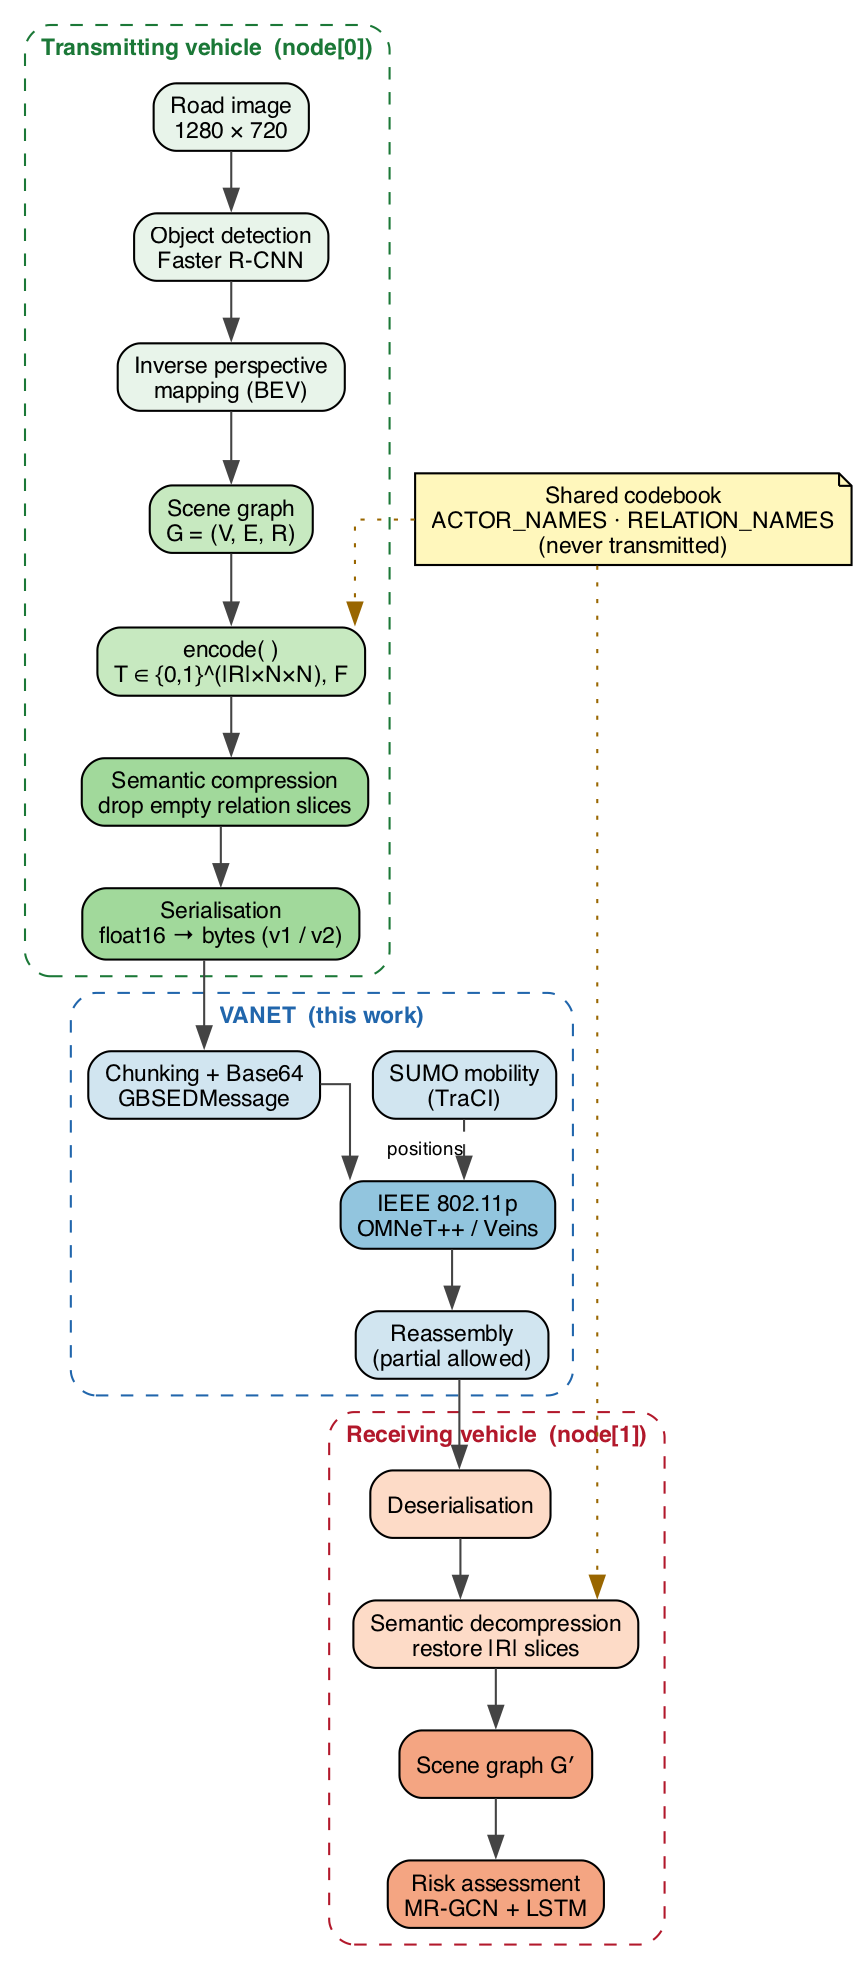
\includegraphics[height=0.82\textheight]{figures/architecture.png}
    \caption{The GBSED semantic chain integrated with a VANET simulation. Green
    is the transmitting vehicle, blue the network contribution of this project,
    red the receiving vehicle. The shared codebook is never transmitted: node
    names are re-derived at the receiver from label indices.}
    \label{fig:architecture}
\end{figure}

A deliberate architectural decision underlies the whole design: \textbf{the
semantic layer never executes inside the simulation}. Encoding is a
pre-process, decoding a post-process, and the network moves opaque bytes
between them. This is justified because the encoder's output depends on nothing
the simulation knows --- the same image yields the same bytes regardless of
where the vehicles are. Executing it in-loop would add approximately one second
of wall-clock time per frame to a simulation that otherwise completes in
$0.3$\,s, and would buy nothing. The exception, discussed in
Chapter~\ref{chapter:conclusion}, is adaptive encoding, where the transmitter
chooses what to send based on live link quality.

\section{Chronological Breakdown of Components}

\subsection{Layer 1: Image to Scene Graph}

An object detector localises road entities. The published implementation uses
Detectron2's Mask R-CNN, which requires CUDA; we substitute torchvision's
Faster R-CNN \cite{ren2015faster}, which produces the same
(boxes, labels, image size) triple and runs on CPU. Bounding boxes are
projected into a bird's eye view by inverse perspective mapping, and
\texttt{roadscene2vec} constructs the graph: a fixed skeleton of a road node,
an ego node and three lane nodes, plus one node per detected actor, connected
by relations determined by distance and bearing thresholds.

\subsection{Layer 2: Semantic Encoding and Compression}

The graph is encoded as an adjacency tensor
$T \in \{0,1\}^{|R| \times N \times N\!}$ over $|R| = 12$ relation types and
$N$ nodes, plus a node feature matrix $F$. Semantic compression removes every
relation slice that is entirely zero, yielding a compressed tensor $T'$ and an
index list $L$ recording which relations survived. For the scenes in this study
this discards between $4$ and $8$ of the $12$ slices.

\subsection{Layer 3: Serialisation}

The arrays are flattened into a single \texttt{float16} vector, each section
preceded by its length, and written as bytes. We refer to this as format
\textbf{v1}; it is byte-for-byte identical to the published implementation.

\subsection{Layer 4: Transport}

The payload is split into fixed-size chunks, Base64-encoded, and broadcast as
802.11p Wave Short Messages. The receiver reassembles them.

\subsection{Layer 5: Decoding and Task Inference}

Deserialisation, semantic decompression and graph regeneration reverse the
encoder. The reconstructed graph feeds an MR-GCN with an LSTM and attention
layers for sequence-level risk classification.

\section{The Fixed-Budget Comparison}

The central methodological contribution is the design of a \emph{controlled}
comparison against a pixel baseline. Three arms are constructed:

\begin{description}
    \item[Full image.] The original JPEG, transmitted as-is. This answers a
    feasibility question.
    \item[Matched budget.] Each image is re-encoded --- by searching over scale
    and quality --- to the largest representation that fits within \emph{that
    frame's exact GBSED payload size}. Identical bytes produce an identical
    chunk count, hence identical packets over an identical channel. Delivery is
    therefore identical by construction, and any difference in outcome is
    attributable to the representation alone.
    \item[Budget sweep.] The budget is then multiplied by $1, 2, 4, \ldots, 128$
    and the measurement repeated without a channel, producing a
    rate--semantics curve.
\end{description}

Both arms run the same detector, the same graph extraction and the same scoring
code. The received image is upscaled to $1280 \times 720$ before detection ---
not a handicap but a requirement, since the BEV homography and the distance
thresholds are calibrated for that resolution.

\subsection{Validity control}

The budget sweep includes the original, unbounded-budget image as a reference
point. Because the ground-truth graphs were themselves produced from those
images, the image arm \emph{must} score $1.000$ there. Verifying that it does
is what distinguishes a genuine bitrate effect from a defect in the image
pipeline.

\section{Evaluation Metrics}

Four metrics are used, defined once and applied identically to both arms.

\begin{description}
    \item[Delivery rate.] Fraction of frames that arrived at all. A property of
    the channel, not the representation.
    \item[Graph-exact rate.] Fraction of frames whose reconstruction is node-
    and edge-identical to the original.
    \item[Actor-edge F1.] F1 over edges with at least one detected actor at an
    end. This excludes the road/ego/lane skeleton, which is present regardless
    of image content and constitutes roughly $38\%$ of a typical edge set.
    \item[Safety-relation recall.] The fraction of \texttt{near\_coll} and
    \texttt{super\_near} relations involving the ego vehicle that survive.
    This is the content a braking decision actually reads.
\end{description}

\section{Summary of the Methodology}

The method is to hold the channel, the frames, the detector, the extraction and
the scoring constant, and vary exactly one thing --- what the transmitted bytes
represent. Every claim in Chapter~\ref{chapter:results} rests on that control.

%============================================================================
\chapter{Implementation} \label{chapter:impl}
%============================================================================

\section{Technology Stack}

\begin{table}[htbp]
\centering
\begin{tabular}{l l l}
\toprule
\textbf{Component} & \textbf{Technology} & \textbf{Version} \\
\midrule
Network simulator & OMNeT++ \cite{varga2008overview} & 6.4.0 \\
VANET framework & Veins \cite{sommer2011bidirectionally} & 5.3.1 \\
Traffic simulator & SUMO \cite{lopez2018microscopic} & 1.21.0 \\
Physical layer & IEEE 802.11p \cite{ieee80211p} & 6\,Mbit/s, 20\,mW \\
Scene graphs & \texttt{roadscene2vec} \cite{malawade2022roadscene2vec} & --- \\
Object detection & torchvision Faster R-CNN \cite{ren2015faster} & 0.23.0 \\
Deep learning & PyTorch / PyTorch Geometric & 2.8.0 \\
Application layer & C++17 & --- \\
Tooling & Python & 3.12 \\
\bottomrule
\end{tabular}
\caption{Technology stack.}
\label{tab:stack}
\end{table}

\section{The Veins Application}

\texttt{GBSEDApp} extends Veins' \texttt{DemoBaseApplLayer}. The sender loads a
queue of payload files, splits each into chunks, Base64-encodes them and
broadcasts them as \texttt{GBSEDMessage} frames carrying the chunk index, the
total chunk count, the file name and the sender's position. The receiver
allocates a buffer on the first chunk of a file and writes the reassembled
result to disk.

Several extensions were required.

\textbf{Configurable timing.} The send interval and start time were hard-coded
constants, which made the transmittable volume a property of the source code
rather than of the experiment. Both are now NED parameters.

\textbf{Position stamping and logging.} Each message now carries the sender's
coordinates so the receiver can compute the separation at reception. Both nodes
append one row per chunk to \texttt{tx\_log.csv} and \texttt{rx\_log.csv},
which is what makes delivery analysable against distance.

\textbf{Partial file delivery.} The receiver previously discarded any file that
never completed, making a frame missing one chunk indistinguishable from a
frame never sent. It now writes incomplete files, zero-filled where chunks are
missing --- a precondition for the slice-aligned format below.

\section{The Semantic Tooling}

The semantic layer was consolidated into a single importable module,
\texttt{gbsed\_semantic.py}. This matters because the serialisation functions
had previously been duplicated verbatim between the pipeline script and an
exploratory notebook, an arrangement guaranteed to drift. Two command-line
tools wrap it: an encoder that turns a folder of images into payloads plus
ground-truth metadata, and a decoder that rebuilds graphs from received bytes
and scores them.

\section{The Slice-Aligned Payload Format (v2)}

Semantic decompression already tolerates a partial relation set: it writes each
delivered slice to its index in $T$ and leaves the remainder zero, and cannot
distinguish ``this relation was absent from the scene'' from ``this relation's
slice did not arrive''. The capability existed; only the packing discarded it.

Format v2 builds the payload as a whole number of blocks of exactly
\texttt{chunkSize} bytes. Each block begins with a magic number and carries
only \emph{complete} relation slices; block~0 additionally carries the node
block. Because the transport chunks naively at the same size, every network
chunk is one self-contained block. A missing block is all zeros, fails the
magic check and is skipped.

Slices are ordered safety-first. An earlier ordering that led with the
structural \texttt{isIn} relation pushed \texttt{near\_coll} into block~1 at
small chunk sizes, where losing one chunk cost every safety relation --- the
exact failure the format exists to prevent.

The decoder's core required no modification: \texttt{decode()} is simply called
with whatever index list survived.

\section{Verification}

\begin{itemize}
    \item Format v1 remains the default and still round-trips byte-identically
    through the published serialiser for all 20 frames.
    \item Format v2 produces identical scene graphs to v1 (0 of 20 differ).
    \item A drop-one-block test over every block confirms that losing block~0
    yields a clean diagnostic error while losing any other block recovers
    $5/7$ relations with safety relations intact.
    \item The Baseline configuration was reproduced independently on macOS and
    Linux, returning $14/20$ delivered on both.
\end{itemize}

%============================================================================
\chapter{Results and Discussion} \label{chapter:results}
%============================================================================

\section{Datasets and Experimental Setup}

Two sequences of consecutive frames from a lane-change driving dataset were
used: \texttt{seq1} (20 frames) and \texttt{seq2} (23 frames), at
$1280 \times 720$. Scene graphs contain 6--10 nodes, and payloads range from
$436$ to $1642$ bytes with a mean of $811$.

The SUMO scenario places two vehicles at a common junction travelling at right
angles at $8$\,m/s, so their separation grows continuously and the sequence
crosses the radio range limit mid-run. At this speed both vehicles outlive the
send queue, so delivery is governed by distance alone rather than by the sender
disappearing. Figure~\ref{fig:scenario} shows the geometry and the measured
result.

\begin{figure}[htbp]
    \centering
    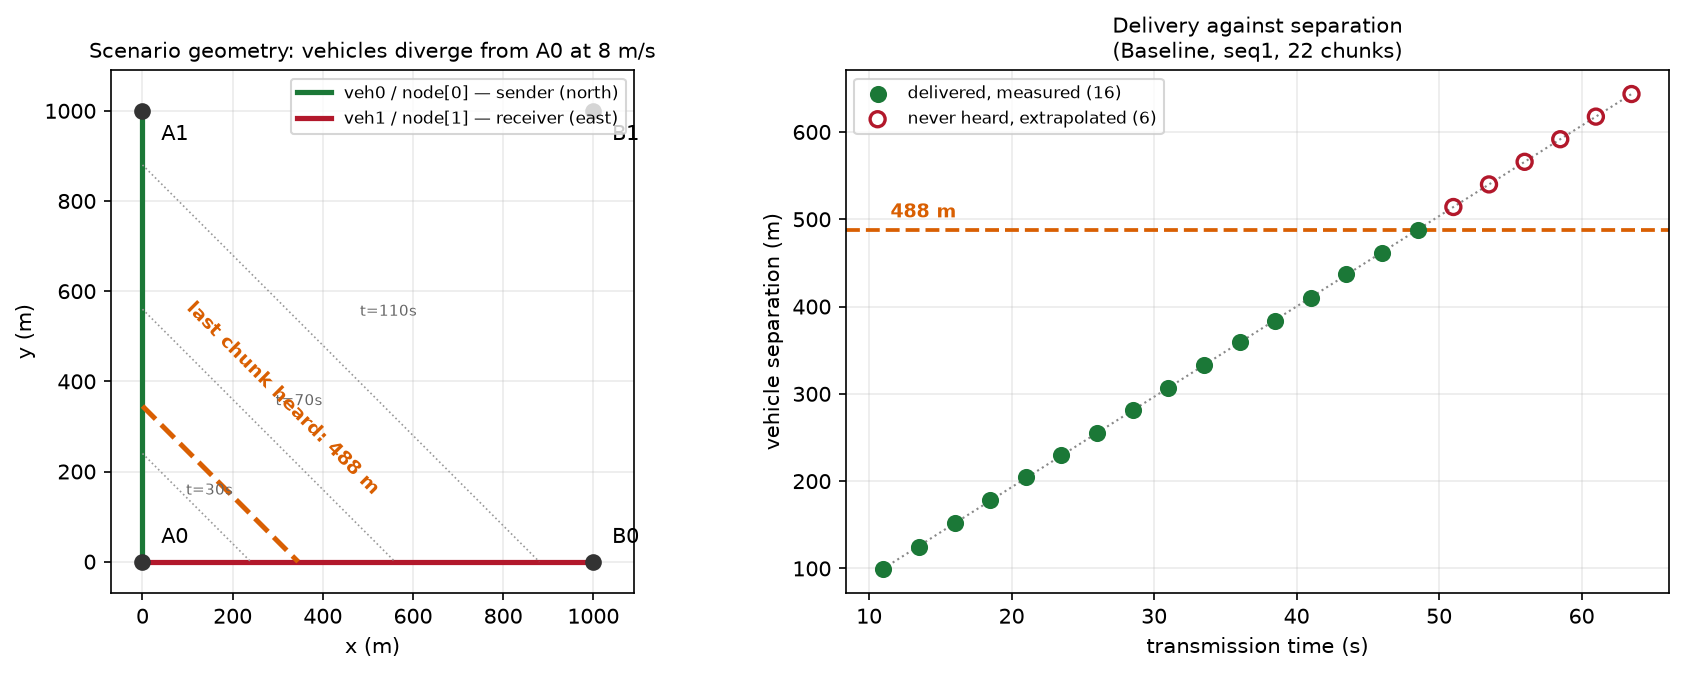
\includegraphics[width=\textwidth]{figures/scenario.png}
    \caption{Left: scenario geometry. Right: measured delivery against vehicle
    separation. Separation grows at $10.35$\,m/s ($r = 0.99999$ against the
    app's own logged distances); the last chunk heard was at $488$\,m.}
    \label{fig:scenario}
\end{figure}

Five channel conditions were evaluated by varying the receiver noise floor from
$-98$ to $-80$\,dBm.

\section{Semantic Fidelity over a Real Network}

The first result is that the chain survives the port. Across both sequences and
all conditions, \textbf{every delivered frame reconstructed
node- and edge-identically}: actor-edge F1 of $1.000$ and safety-relation
recall of $1.000$ on delivered frames, in every configuration.
Figure~\ref{fig:qualitative} shows a representative frame.

\begin{figure}[htbp]
    \centering
    \begin{subfigure}[b]{0.49\textwidth}
        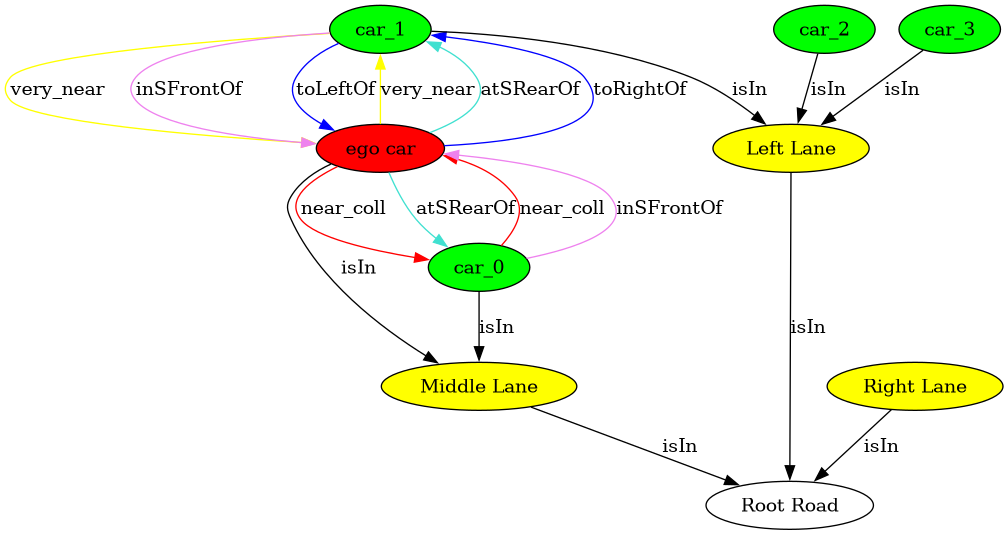
\includegraphics[width=\textwidth]{figures/sg_original.png}
        \caption{Transmitted}
    \end{subfigure}
    \hfill
    \begin{subfigure}[b]{0.49\textwidth}
        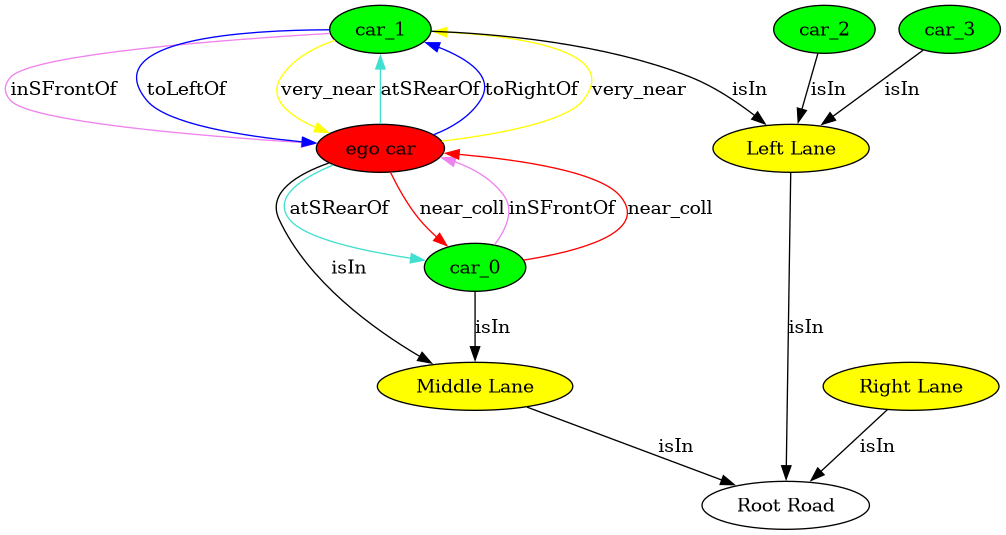
\includegraphics[width=\textwidth]{figures/sg_reconstructed.png}
        \caption{Reconstructed at the receiver}
    \end{subfigure}
    \caption{A five-actor scene graph before transmission and after
    reconstruction, delivered at $461$\,m. Node names, lane structure and all
    relations are recovered exactly, although names are never transmitted.}
    \label{fig:qualitative}
\end{figure}

This is a stronger statement than the original SNR study can make. Because
802.11p either delivers a frame with a valid checksum or drops it entirely,
there is no partially corrupted payload: fidelity is either perfect or the
frame is absent. Semantic degradation in a VANET is therefore a question of
\emph{which frames arrive}, not of how damaged they are.

\section{The Fixed-Budget Comparison}

Table~\ref{tab:matched} and Figure~\ref{fig:matched} give the central result.

\begin{table}[htbp]
\centering
\begin{tabular}{l l r r r r}
\toprule
\textbf{Arm} & \textbf{Config} & \textbf{Delivered} & \textbf{Graph exact} & \textbf{Safety kept} & \textbf{Actor F1} \\
\midrule
GBSED            & Baseline     & 70\% & \textbf{70\%} & \textbf{32/32} & \textbf{1.000} \\
GBSED            & Noise\_Low   & 55\% & 55\%          & 24/24          & 1.000 \\
GBSED            & Noise\_Medium& 25\% & 25\%          & 8/8            & 1.000 \\
\midrule
WebP @ budget    & Baseline     & 70\% & \textbf{0\%}  & \textbf{0/32}  & \textbf{0.000} \\
WebP @ budget    & Noise\_Low   & 55\% & 0\%           & 0/24           & 0.000 \\
JPEG @ budget    & Baseline     & 70\% & \textbf{0\%}  & \textbf{0/32}  & \textbf{0.000} \\
JPEG @ budget    & Noise\_Low   & 55\% & 0\%           & 0/24           & 0.000 \\
\bottomrule
\end{tabular}
\caption{Matched-budget comparison. Delivery is identical across arms by
construction; only the representation differs.}
\label{tab:matched}
\end{table}

\begin{figure}[htbp]
    \centering
    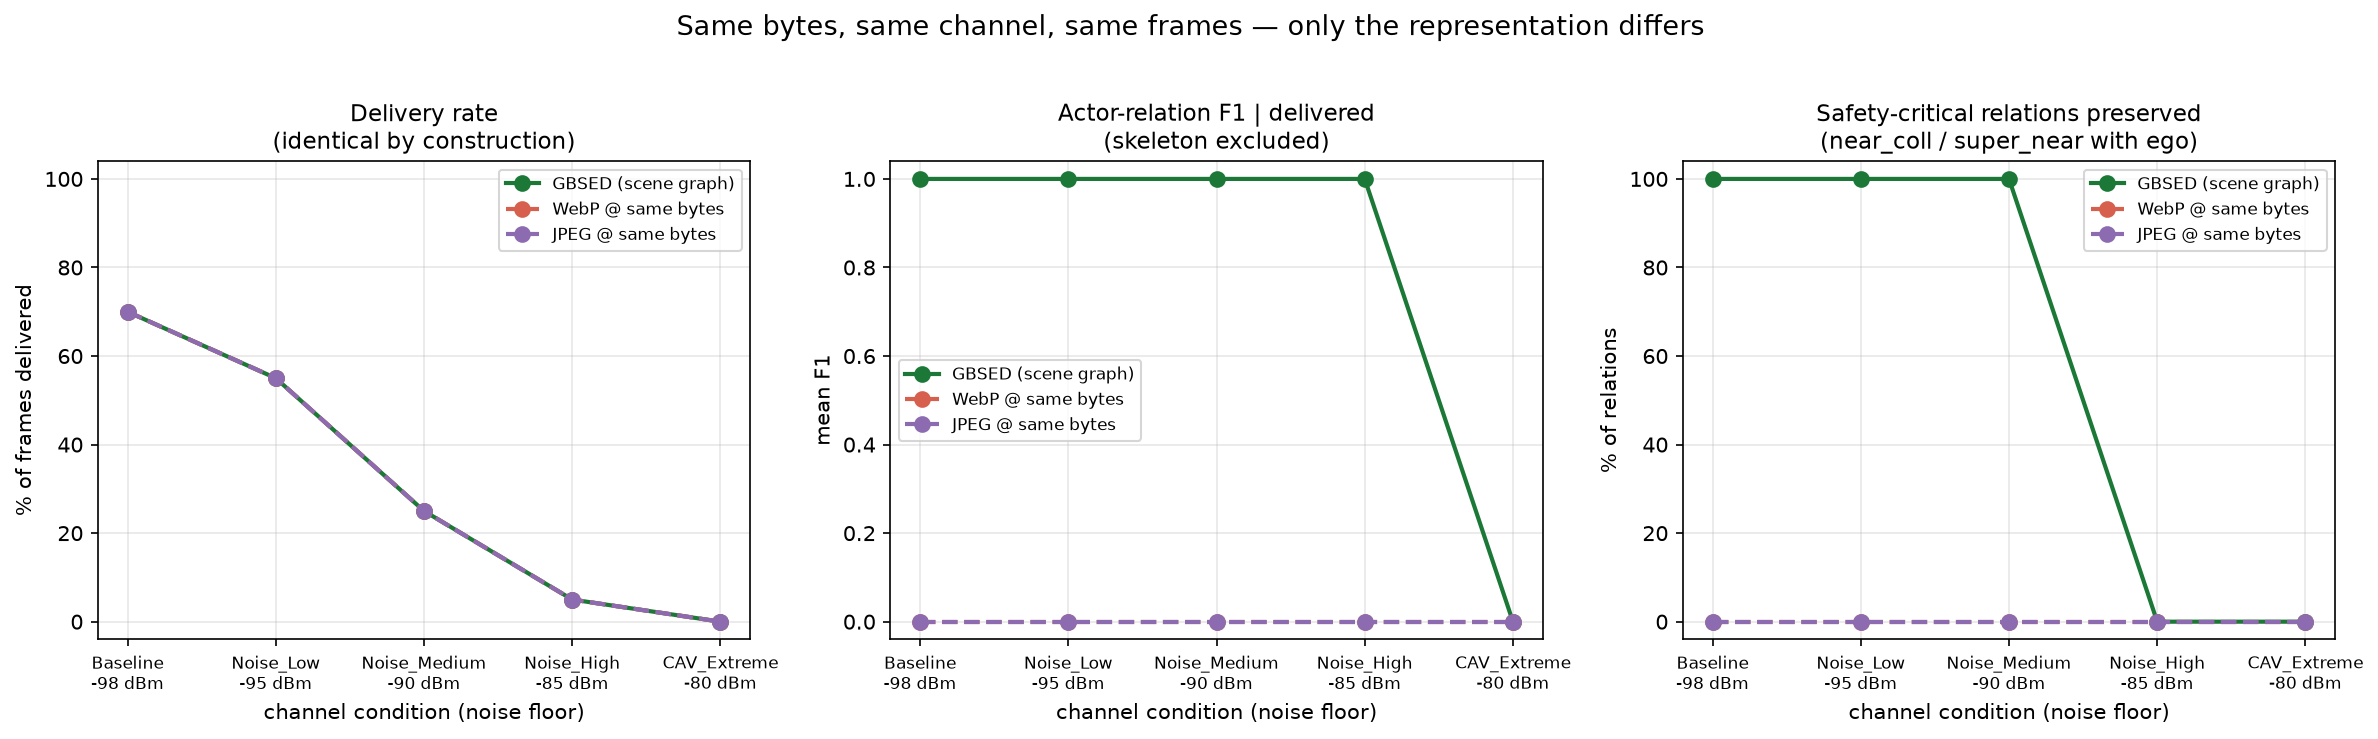
\includegraphics[width=\textwidth]{figures/matched_budget.png}
    \caption{Same bytes, same channel, same frames. The three overlapping lines
    in the left panel confirm the control held. The other two panels show the
    consequence.}
    \label{fig:matched}
\end{figure}

At the GBSED byte budget, an image is $102 \times 58$ to $256 \times 144$
pixels at quality 1--5. Across the 14 frames delivered on the best channel the
detector found 18 objects in the WebP frames and \emph{zero} in the JPEG
frames, against roughly 40 in the originals. Not one of the 32 safety-critical
relations survived in either codec.

WebP was given every advantage --- it is markedly better than JPEG at very low
bitrate, it came in \emph{under} budget ($14{,}604$\,B against GBSED's
$16{,}218$), and it held $256 \times 144$ where JPEG collapsed to
$102 \times 58$. It still recovered nothing.

\subsection{Transmitting the whole frame}

For completeness, Table~\ref{tab:full} reports the naive baseline. The result
is not that it is wasteful but that it is impossible: on the best channel the
receiver heard 16 chunks, all belonging to frame~0, which requires 1{,}295 ---
$1.24\%$ of a single frame.

\begin{table}[htbp]
\centering
\begin{tabular}{l r r}
\toprule
 & \textbf{GBSED} & \textbf{Full JPEG} \\
\midrule
Total bytes, 20 frames      & 16{,}218 & 24{,}839{,}399 ($1531\times$) \\
Chunks at 1000\,B           & 22       & 24{,}847 \\
Simulated time to send      & 55\,s    & 62{,}118\,s (17.3 hours) \\
Sender vehicle lifetime     & 125\,s   & 125\,s \\
Frames delivered (Baseline) & 14/20    & \textbf{0/20} \\
\bottomrule
\end{tabular}
\caption{The full-image baseline. Payload sizes are also shown in
Figure~\ref{fig:payload}.}
\label{tab:full}
\end{table}

\begin{figure}[htbp]
    \centering
    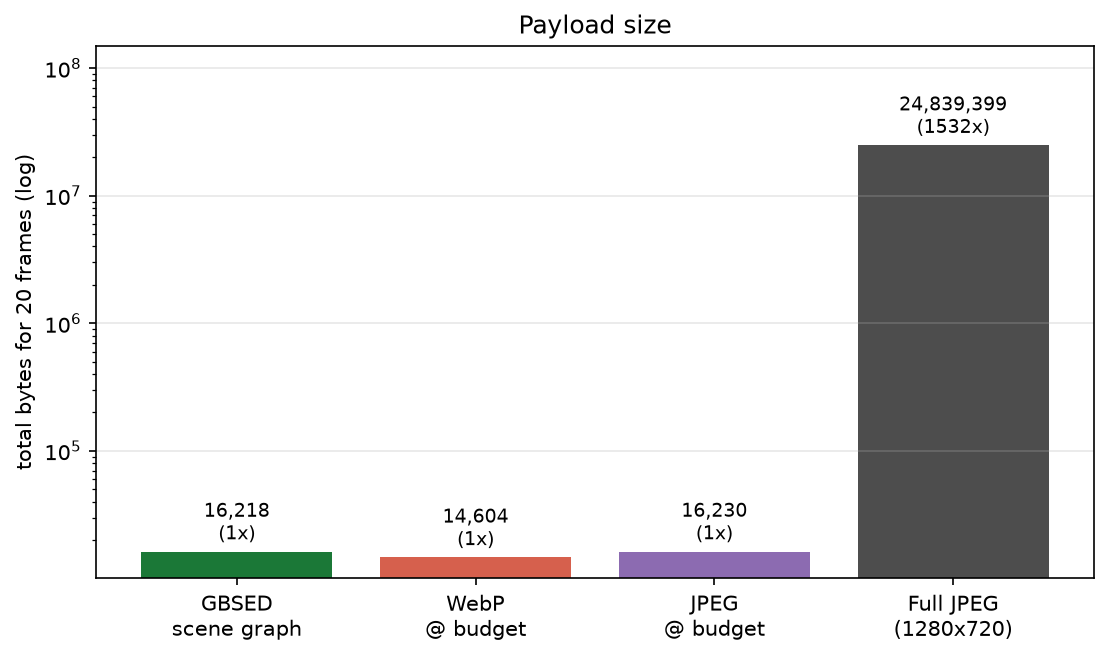
\includegraphics[width=0.7\textwidth]{figures/payload_size.png}
    \caption{Total payload for 20 frames, log scale.}
    \label{fig:payload}
\end{figure}

\section{The Rate--Semantics Curve}

The matched-budget result invites the question of how much more bandwidth
pixels would need. Figure~\ref{fig:rate} and Table~\ref{tab:sweep} answer it.

\begin{figure}[htbp]
    \centering
    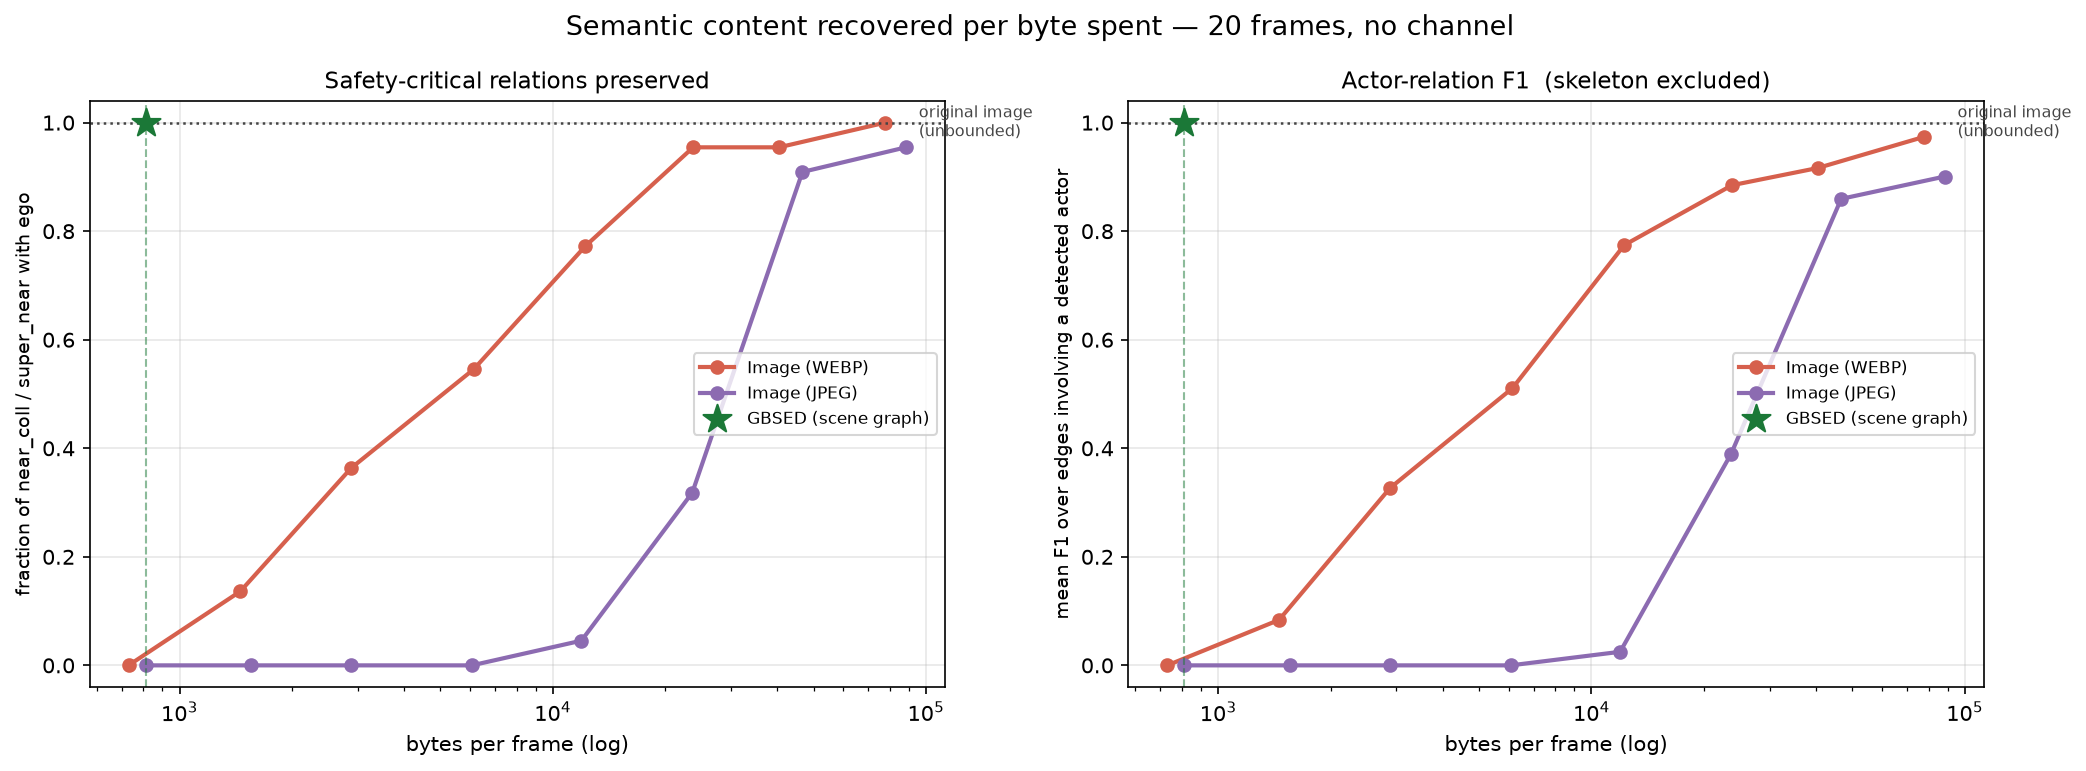
\includegraphics[width=\textwidth]{figures/rate_semantics.png}
    \caption{Semantic content recovered per byte spent, channel-free. GBSED is
    the green star at $811$\,B. The dotted line is the original image at
    unbounded budget --- the arm's validity control, which it reaches.}
    \label{fig:rate}
\end{figure}

\begin{table}[htbp]
\centering
\begin{tabular}{l r r r r r}
\toprule
\textbf{Budget} & \textbf{Bytes/frame} & \textbf{WebP safety} & \textbf{WebP F1} & \textbf{JPEG safety} & \textbf{JPEG F1} \\
\midrule
$\times 1$   & 800     & 0/44  & 0.000 & 0/44  & 0.000 \\
$\times 2$   & 1{,}500 & 6/44  & 0.084 & 0/44  & 0.000 \\
$\times 4$   & 2{,}900 & 16/44 & 0.327 & 0/44  & 0.000 \\
$\times 8$   & 6{,}100 & 24/44 & 0.511 & 0/44  & 0.000 \\
$\times 16$  & 12{,}100& 34/44 & 0.774 & 2/44  & 0.025 \\
$\times 32$  & 23{,}700& 42/44 & 0.885 & 14/44 & 0.389 \\
$\times 64$  & 43{,}500& 42/44 & 0.916 & 40/44 & 0.860 \\
$\times 128$ & 83{,}000& \textbf{44/44} & 0.974 & 42/44 & 0.901 \\
\midrule
\textbf{GBSED} & \textbf{811} & \textbf{44/44} & \textbf{1.000} & --- & --- \\
\bottomrule
\end{tabular}
\caption{Rate--semantics sweep. WebP first matches GBSED's safety-relation
recall at $77{,}809$\,B/frame, i.e.\ $96\times$. JPEG does not reach it within
the sweep.}
\label{tab:sweep}
\end{table}

Expressed as efficiency, GBSED spends $369$ bytes per preserved safety
relation; WebP at the budget where it finally matches spends $35{,}368$.

The shape of the curves is itself informative. JPEG sits at exactly $0.000$
through $\times 8$ and then rises steeply. Image codecs degrade
\emph{uniformly}: every object blurs together, and below a threshold the
detector fails on all of them at once. That cliff is the mechanism made
visible.

\section{Graceful Degradation via Slice-Aligned Packing}

\begin{figure}[htbp]
    \centering
    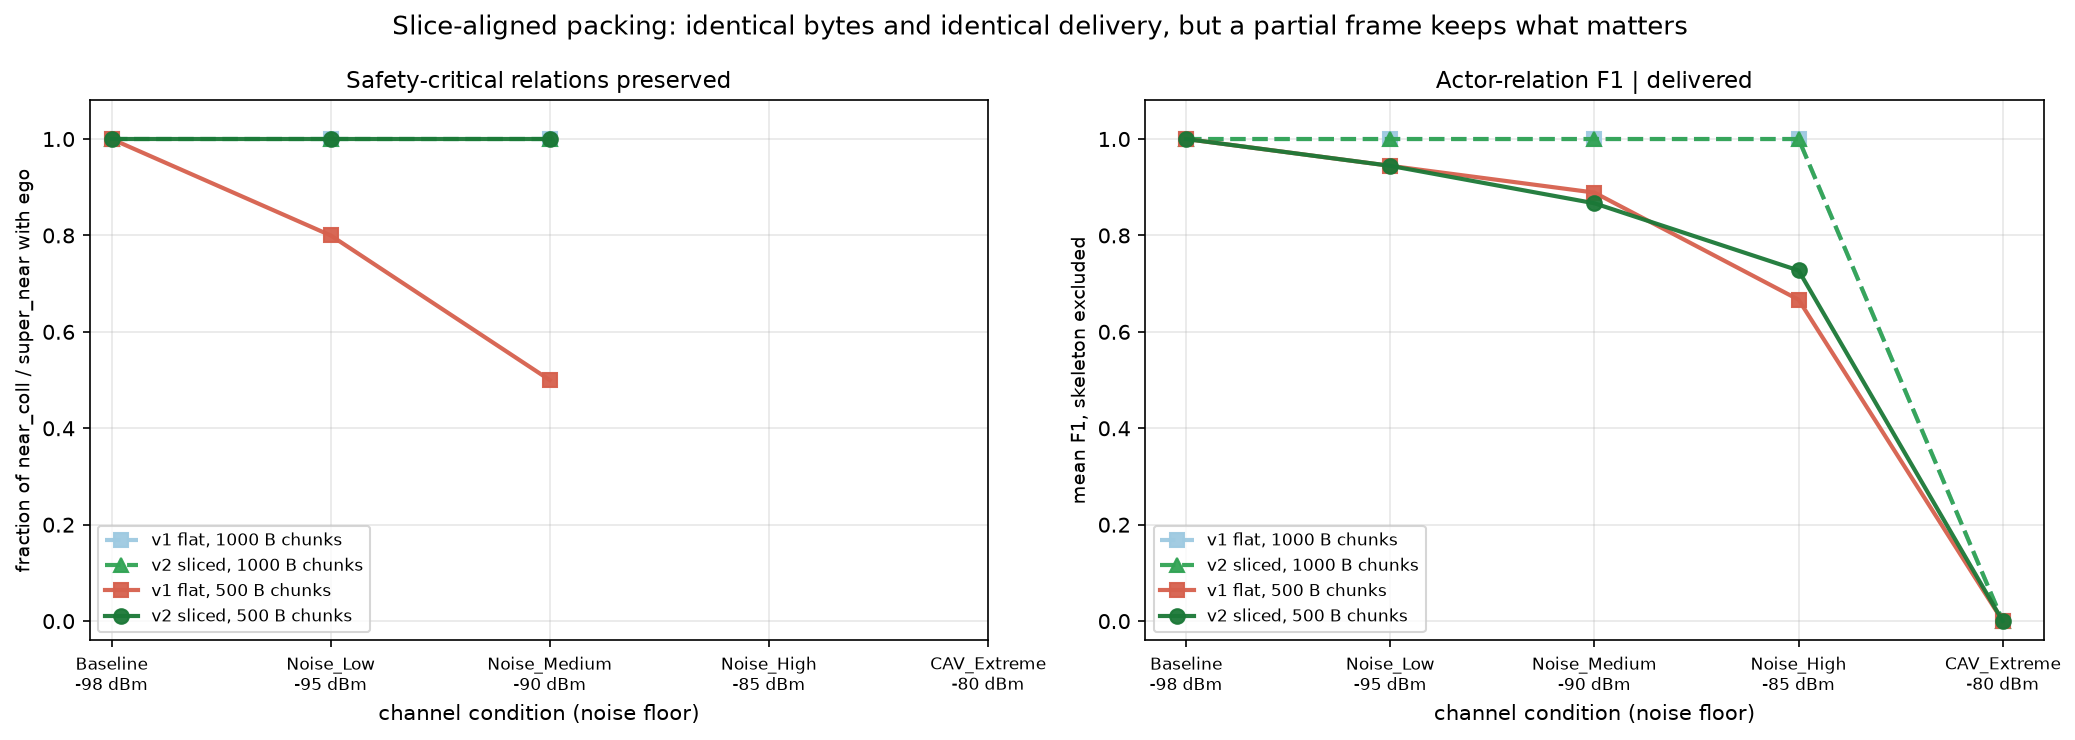
\includegraphics[width=\textwidth]{figures/format_sweep.png}
    \caption{Format v1 against v2. The 1000\,B pair coincide because only 2 of
    20 frames span more than one chunk at that size. The 500\,B pair separate:
    v1 falls to $0.80$ then $0.50$; v2 holds $1.00$.}
    \label{fig:format}
\end{figure}

At $500$-byte chunks, where frames genuinely span blocks, safety-relation
recall under partial delivery rises from $0.80$ and $0.50$ (v1) to $1.00$ and
$1.00$ (v2) at Noise\_Low and Noise\_Medium respectively --- with identical
bytes, identical delivery, and zero additional chunks on the wire at
$1000$\,B, one additional at $500$\,B.

A single frame illustrates the mechanism. It received 1 of its 2 chunks under
both formats:

\begin{center}
\begin{tabular}{l l l}
\toprule
 & \textbf{Safety relations} & \textbf{Reported as} \\
\midrule
v1 & $0/2$ & ``payload differs from sent bytes'' \\
v2 & $\mathbf{2/2}$ & ``partial: 1 block lost, 3/7 relations recovered'' \\
\bottomrule
\end{tabular}
\end{center}

Same bytes on the air, same chunk lost. v1 loses both safety relations; v2
keeps both \emph{and reports precisely what is missing}.

\section{Corrected Evaluation Defects}

Three defects in the inherited evaluation were identified and corrected. They
are reported here because each would have distorted the conclusions.

\subsection{Three metrics that were one number}

In every row of the original results, delivery rate, bit-exact rate and mean
edge F1 were identical (Figure~\ref{fig:superseded}). Two distinct causes:

\textbf{Bit-exact rate $\equiv$ delivery rate} is real, not a bug. IEEE 802.11p
delivers a frame with a valid checksum or drops it, so a delivered frame is
always bit-exact. The column is worth keeping only as an assertion that should
never fire.

\textbf{Mean edge F1 $\equiv$ delivery rate} was a genuine defect. The
aggregation filtered lost frames with \texttt{if r["edge\_f1"]}, but their
value is the \emph{string} \texttt{"0.0"}, which is truthy in Python. Lost
frames entered the mean as zeros, and since every delivered frame scores
exactly $1.0$, the mean collapsed to the delivery rate.

\begin{figure}[htbp]
    \centering
    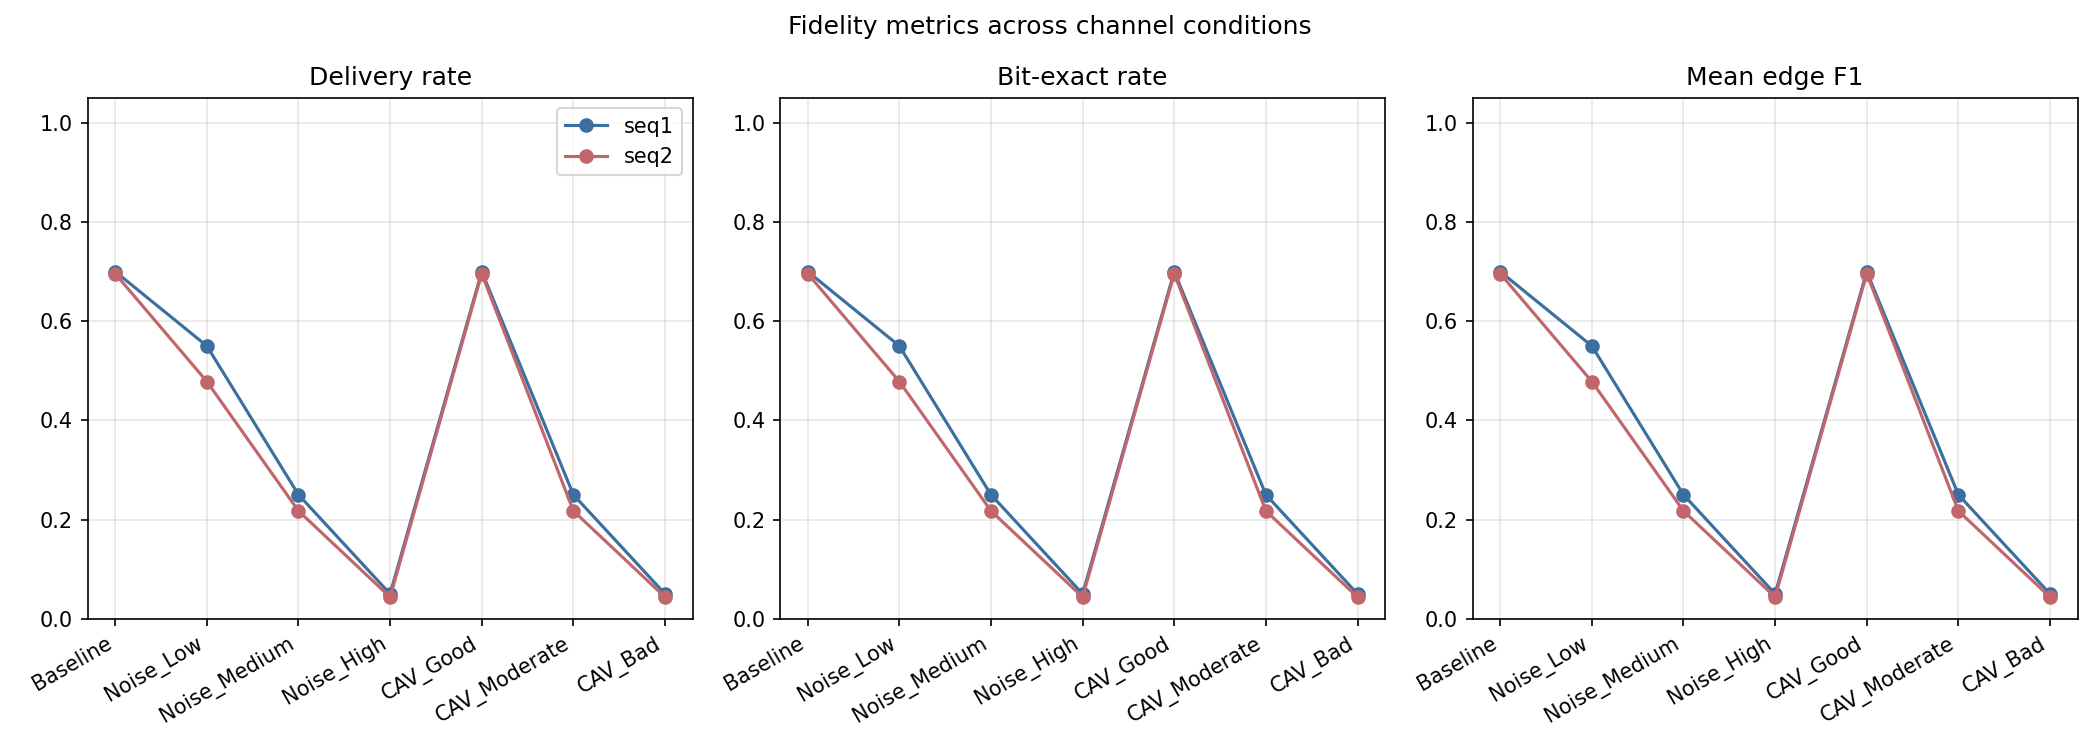
\includegraphics[width=\textwidth]{figures/superseded_metrics.png}
    \caption{The superseded figure, retained as evidence. Three panels plot the
    identical curve, and the rise at \texttt{CAV\_Good} is not a recovery but
    \texttt{Baseline} replotted under a duplicate configuration.}
    \label{fig:superseded}
\end{figure}

\subsection{A metric floor of 0.38}

The JPEG arm scored $0.386$ mean edge F1 on the best channel \emph{with zero
detections}. Every graph contains a road node, an ego node and three lanes
joined by \texttt{isIn} edges regardless of image content, and that skeleton is
roughly $38\%$ of the edge set. Edge F1 therefore ranged over $[0.38, 1]$, with
the bottom meaning ``understood nothing''. The actor-edge F1 metric introduced
in Chapter~\ref{chapter:proposed} reads $0.000$ for the same input.

\subsection{Three duplicate channel configurations}

Three of the eight configurations differed from three others only by
\texttt{*.node[1].veinsmobility.x}. That parameter has no effect: node
positions come from SUMO over TraCI and are overwritten at every update. The
evidence is bit-identical classifier output --- \texttt{prob\_class1} of
$0.9753320813179016$ for both \texttt{Baseline} and \texttt{CAV\_Good} ---
which can only arise from identical input graphs. Eight configurations were
really five noise floors.

This also biased the accuracy summary, since accuracy was computed over
configurations and duplicated conditions were counted twice:
\texttt{seq1} read $3/7 = 0.43$ where the deduplicated value is $2/4 = 0.50$.

\section{Interpreting the Results: Why GBSED Works}

Three separable mechanisms explain the gap, and they are worth distinguishing
because they are usually collapsed into ``compression''.

\textbf{It compresses the right thing.} A JPEG spends bits on texture,
lighting, road surface and sky, none of which the risk classifier reads. The
scene graph spends them on actor identity, position and pairwise relations,
which is exactly what it consumes. The $1531\times$ reduction is not a better
codec; it is a change in what counts as signal.

\textbf{It degrades in a different dimension.} Image codecs degrade spatially
and uniformly, producing the cliff visible in Figure~\ref{fig:rate}. A scene
graph decomposes into independent relation slices, so bits removed cost
relation categories rather than everything at once --- as demonstrated in
Figure~\ref{fig:format}.

\textbf{Semantic content is discrete.} A relation is a binary edge; node labels
are small integers. These are exactly representable in \texttt{float16} and are
either right or wrong --- there is no ``slightly wrong \texttt{near\_coll}''.
Pixels are continuous and every bit removed degrades them. This is why every
delivered GBSED frame scores exactly $1.000$ and never $0.98$.

\textbf{The honest framing.} GBSED is not better compression. It transmits the
\emph{output} of perception rather than its \emph{input}, and wins because the
receiver's task needs only that output. The corollary is the limitation: the
receiver can never do anything the sender's extractor did not already encode. A
raw image is task-agnostic; a scene graph is committed. The comparison is fair
only because the downstream task was fixed in advance.

%============================================================================
\chapter{Ethical, Social, and Environmental Considerations} \label{chapter:ethics}
%============================================================================

\section{Safety and Accountability}

A semantic communication system for vehicles makes a consequential trade. By
transmitting an interpretation rather than an observation, it commits to that
interpretation being correct. If the sender's detector misses a pedestrian, no
amount of channel reliability will recover them: the receiver has no pixels to
re-examine. Our own measurements make this concrete --- the graph is recovered
perfectly, but it is only ever as good as the perception that produced it.

This has accountability implications. After an incident, a raw video log can be
re-analysed with better models; a transmitted scene graph cannot. Any
deployment should retain local raw data for forensic purposes even while
transmitting only semantics.

\section{Privacy}

Semantic transmission is, incidentally, privacy-preserving. A scene graph
contains object categories and coarse positions; it contains no faces, no
licence plates and no identifiable imagery. Broadcasting ``a car is 4 feet
ahead in the middle lane'' discloses far less about bystanders than
broadcasting the frame that observation came from. This is a genuine ethical
advantage of the approach and deserves to be stated as such.

\section{Environmental and Spectral Sustainability}

Radio spectrum is a shared, finite resource. A vehicle transmitting $1.2$\,MB
per frame occupies airtime that every other vehicle in range is denied. Our
measurement that a single frame would need $17.3$ hours of channel time, while
the semantic payload needs $55$ seconds for twenty frames, is a statement about
spectral efficiency and therefore about how many vehicles a given deployment
can support. Reduced transmission also means reduced radio energy consumption
per unit of useful information.

\section{Equity of Access}

A system whose bandwidth demands are modest can operate on inexpensive,
widely-available radio hardware. A cooperative perception scheme that requires
high-bandwidth links would be available only to premium vehicles, concentrating
its safety benefits among those who need them least. Semantic communication is
comparatively egalitarian in its infrastructure requirements.

%============================================================================
\chapter{Challenges and Limitations} \label{chapter:limits}
%============================================================================

\section{Challenges Encountered}

\textbf{Toolchain assembly.} SUMO version selection was constrained from three
directions at once: Veins 5.3.1 accepts TraCI API versions 15--21, several
macOS wheels link against absent libraries, and the OMNeT++ installation was
managed by a wrapper that refuses to run outside its own shell. A build-blocking
compilation error in upstream Veins also had to be fixed.

\textbf{Silent failures.} Several defects produced plausible wrong answers
rather than errors: the truthy-string metric bug, the ineffective mobility
parameter, and a malformed XML comment in a route file that surfaced in
OMNeT++ as an apparent TraCI version mismatch. Each cost significant debugging
time and each is now documented.

\textbf{Designing a fair comparison.} The first instinct --- transmit the JPEG
--- produces an uninterpretable result. Arriving at the matched-budget design
required recognising that the byte count had to be controlled per frame.

\section{Limitations}

\textbf{No negative class.} Both evaluated sequences are labelled risky. Without
negative examples, classification accuracy cannot distinguish a working model
from one that always predicts ``risky'', and no false-positive rate is
computable. This bounds what the task-level results can claim.

\textbf{Two sequences.} Forty-three frames total is sufficient to establish the
mechanisms reported here but not to claim statistical generality.

\textbf{Two nodes.} The scenario has one sender and one receiver with fixed
roles. Medium access contention among many vehicles --- which is where 802.11p
becomes genuinely difficult --- is untested.

\textbf{The slice-aligned format needs a suitable regime.} At $1000$-byte
chunks only 2 of 20 frames span more than one chunk, so the two formats are
indistinguishable. The benefit requires either smaller chunks or denser scenes.

\textbf{Byte reproducibility.} Re-encoding on a different platform reproduced
17 of 20 payloads byte-identically; the remainder differ by one unit in the last
place of a single \texttt{float16} feature. The extracted graphs were identical
in all 20, so the encoder is reproducible at the level of scene graphs but not
of bytes.

\textbf{No physical-layer comparison.} We evaluate 802.11p, the original work
evaluates MIMU--OFDM with a CDL channel. The two are complementary; we do not
claim one supersedes the other.

%============================================================================
\chapter{Conclusion and Future Work} \label{chapter:conclusion}
%============================================================================

\section{Summary of Key Findings}

This project asked whether a graph-based semantic representation is genuinely
superior to an image at a fixed bit budget, and answered it under experimental
control.

\begin{enumerate}
    \item The GBSED semantic chain operates losslessly across a realistic
    VANET. Every delivered frame reconstructs exactly; in 802.11p, semantic
    degradation is a question of which frames arrive, not how damaged they are.
    \item At an identical byte budget over an identical channel, the scene
    graph preserves $44/44$ safety-critical relations while both image codecs
    preserve $0/44$.
    \item Images require approximately $96\times$ more bandwidth to convey the
    same safety-relevant content. GBSED spends $369$ bytes per preserved safety
    relation against WebP's $35{,}368$.
    \item Transmitting whole frames is infeasible rather than merely expensive:
    $1.24\%$ of one frame arrived within the vehicles' contact window.
    \item Aligning the payload to relation-slice boundaries raises
    safety-relation recall under partial delivery from $0.50$ to $1.00$ at no
    additional airtime cost.
\end{enumerate}

\section{Contributions}

The project contributes a working integration of a published semantic codec
with a realistic vehicular network; a controlled experimental design that
isolates representational advantage from bandwidth advantage; a
rate--semantics curve quantifying the gap; a payload format that exploits the
architecture's latent robustness; and the correction of three evaluation
defects that would otherwise have distorted the reported results.

\section{Future Directions}

\textbf{Adaptive semantic encoding.} The slice-aligned format makes it possible
for the transmitter to choose \emph{which} relation slices to send based on
live link quality --- sending only safety-critical relations when the link is
poor. Because the decision is a cheap integer comparison over precomputed
slices, this requires no machine learning in the simulation loop.

\textbf{Multi-vehicle scenarios.} Extending beyond two nodes would expose
medium access contention and allow study of how semantic payloads share a
channel, including whether their small size materially improves aggregate
throughput.

\textbf{A balanced evaluation set.} Adding sequences without risk events would
permit a genuine accuracy, precision and recall evaluation of the downstream
task.

\textbf{Closing the loop into SUMO.} Having the receiving vehicle act on the
decoded graph --- braking or rerouting --- would turn the study from a
communication evaluation into a cooperative-perception one.

\textbf{Integrity protection.} The payload carries no checksum, and the flat v1
format parses a truncated payload without complaint. A CRC field in the message
would close this cleanly.

\section{Concluding Remarks}

The most useful outcome of this work is not the compression figure but the
experimental design that produced it. A compression ratio quoted against raw
pixels answers a question nobody asks. Holding the byte budget, the channel,
the frames and the scoring constant --- and varying only what the bytes mean
--- produces a claim that is considerably harder to argue with, and one that
happens to be far stronger.

%-------------------------- BACK MATTER --------------------------%
\printbib

\begin{appendices}
\chapter{Weekly Meeting Summary}

\begin{table}[h!]
\centering
\renewcommand{\arraystretch}{1.3}
\setlength{\tabcolsep}{4pt}
\begin{tabular}{|p{0.9cm}|p{1.8cm}|p{2.3cm}|p{2.3cm}|p{2.3cm}|p{2.2cm}|}
\hline
\textbf{Serial} & \textbf{Date} & \textbf{Member 1 Contribution} & \textbf{Member 2 Contribution} & \textbf{Member 3 Contribution} & \textbf{Next Plan} \\ \hline
 &  &  &  &  &  \\ \hline
\end{tabular}
\caption{Group Contribution and Next Plan Table}
\end{table}

\textit{<<Fill from your meeting records.>>}

\chapter{Code and Implementation Artifacts}

\section{Repositories}

\begin{itemize}
    \item Semantic layer, tooling and experiments:\\
    \url{https://github.com/sahil0319/gbsed}
    \item Veins application and simulation scenario:\\
    \url{https://github.com/Loona6/gbsed_veins}
\end{itemize}

\section{Quantitative Summary: GitHub Metrics}

\begin{table}[h]
    \centering
    \caption{Developer Contribution Metrics. \textit{<<Verify against GitHub Insights before submission.>>}}
    \label{tab:metrics}
    \begin{tabular}{l c c c}
        \toprule
        \textbf{Team Member} & \textbf{Total Commits} & \textbf{Additions} & \textbf{Deletions} \\
        \midrule
        <<Member 1>> & <<\ >> & <<\ >> & <<\ >> \\
        <<Member 2>> & <<\ >> & <<\ >> & <<\ >> \\
        <<Member 3>> & <<\ >> & <<\ >> & <<\ >> \\
        \bottomrule
    \end{tabular}
\end{table}

\section{Feature Ownership and Technical Contribution}

\textit{<<Assign the features below to the responsible member.>>}

\begin{center}
\begin{tabular}{|>{\centering\arraybackslash}m{2.6cm}|p{11.5cm}|}
    \hline
    \textbf{Team Member} & \textbf{Technical Summary} \\
    \hline
    <<Member 1>> & \textbf{Veins application layer.} Extended \texttt{GBSEDApp} with configurable send timing, sender position stamping, per-chunk CSV logging, and partial-file delivery. Reworked the SUMO scenario so the two vehicles diverge, converting a trivially lossless link into a measurable range sweep. \\
    \hline
    <<Member 2>> & \textbf{Semantic tooling and experiment harness.} Consolidated the duplicated serialisation code into \texttt{gbsed\_semantic.py}; built the encoder and decoder command-line tools, the channel-configuration sweep, and the risk-assessment integration. \\
    \hline
    <<Member 3>> & \textbf{Pixel baseline and evaluation metrics.} Designed and implemented the matched-budget image baseline and the rate--semantics sweep; introduced actor-edge F1 and safety-relation recall, and diagnosed the three evaluation defects reported in Chapter~\ref{chapter:results}. \\
    \hline
\end{tabular}
\end{center}

\section{Verification: GitHub Screenshots}

\begin{figure}[h]
    \centering
    \framebox{\parbox{0.9\textwidth}{\centering
      \vspace{2.5cm}
      \textbf{Image Placeholder: GitHub Commits Page Screenshot} \\
      \small\textit{Insert screenshot of the repository's 'Commits' history page.}
      \vspace{2.5cm}
    }}
    \caption{GitHub commit history.}
    \label{fig:commits}
\end{figure}

\begin{figure}[h]
    \centering
    \framebox{\parbox{0.9\textwidth}{\centering
      \vspace{2.5cm}
      \textbf{Image Placeholder: GitHub Contributors Graph Screenshot} \\
      \small\textit{Insert screenshot of Insights $\rightarrow$ Contributors.}
      \vspace{2.5cm}
    }}
    \caption{GitHub contributors graph.}
    \label{fig:graph}
\end{figure}

\end{appendices}

\end{document}
